\documentclass[a4paper,10pt,]{article}

% http://www.jmlr.org/format/format.html
%
% See http://jmlr.org/papers/v18/ for example of JMLR papers from last year
%
% Any additional packages needed should be included after jmlr2e.
% Note that jmlr2e.sty includes epsfig, amssymb, natbib and graphicx,
% and defines many common macros, such as 'proof' and 'example'.
% It also sets the bibliographystyle to plainnat; for more information on
% natbib citation styles, see the natbib documentation, a copy of which
% is archived at http://www.jmlr.org/format/natbib.pdf
\usepackage{jmlr2e}
\usepackage{amsmath}

\usepackage{ifxetex,ifluatex}
\ifnum 0\ifxetex 1\fi\ifluatex 1\fi=0 % if pdftex
  \usepackage[utf8]{inputenc}
  \usepackage[T1]{fontenc}
\else % if luatex or xelatex
  \usepackage{unicode-math}
  \defaultfontfeatures{Ligatures=TeX,Scale=MatchLowercase}
\fi

% use upquote if available, for straight quotes in verbatim environments
\IfFileExists{upquote.sty}{\usepackage{upquote}}{}

% use microtype if available
\IfFileExists{microtype.sty}{%
\usepackage[]{microtype}
\UseMicrotypeSet[protrusion]{basicmath} % disable protrusion for tt fonts
}{}

\usepackage{xcolor}
\definecolor{dkgreen}{rgb}{0,0.4,0}           % Define a new color rgb(0, 102, 0)
\definecolor{gray}{rgb}{0.5,0.5,0.5}          % Define a new color rgb(127, 127, 127)
\definecolor{mauve}{rgb}{0.58,0,0.82}         % Define a new color rgb(147, 0, 209)
\definecolor{darkgreen}{rgb}{0.00,0.70,0.00}  % Define a new color rgb(0,178,0)
\definecolor{gold}{RGB}{255,184,0}  % rgb(255,184,0)

\usepackage{lastpage,fancyhdr}     % customize the headers and footers
\pagestyle{fancy}
    \renewcommand{\headrulewidth}{0.2pt}
    \renewcommand{\footrulewidth}{0.2pt}
    \lhead{\emph{SMPyBandits} presentation paper}
    \rhead{\emph{\today}}
    \lfoot{\href{https://GitHub.com/SMPyBandits/SMPyBandits}{GitHub.com/SMPyBandits/SMPyBandits}}
    \cfoot{\(\thepage/\pageref{LastPage}\)}
    \rfoot{Lilian Besson}

% \usepackage{graphicx}
\usepackage{subcaption}
\graphicspath{{../}}
\DeclareGraphicsExtensions{.jpg,.pdf,.mps,.eps,.png}

\IfFileExists{parskip.sty}{%
\usepackage{parskip}
}{% else
\setlength{\parindent}{0pt}
\setlength{\parskip}{6pt plus 2pt minus 1pt}
}
\setlength{\emergencystretch}{3em}  % prevent overfull lines
\providecommand{\tightlist}{%
  \setlength{\itemsep}{0pt}\setlength{\parskip}{0pt}}
\setcounter{secnumdepth}{5}
% Redefines (sub)paragraphs to behave more like sections
\ifx\paragraph\undefined\else
\let\oldparagraph\paragraph
\renewcommand{\paragraph}[1]{\oldparagraph{#1}\mbox{}}
\fi
\ifx\subparagraph\undefined\else
\let\oldsubparagraph\subparagraph
\renewcommand{\subparagraph}[1]{\oldsubparagraph{#1}\mbox{}}
\fi

\usepackage{fancyvrb}
\newcommand{\VerbBar}{|}
\newcommand{\VERB}{\Verb[commandchars=\\\{\}]}
\DefineVerbatimEnvironment{Highlighting}{Verbatim}{commandchars=\\\{\}}
% Add ',fontsize=\small' for more characters per line
\newenvironment{Shaded}{}{}
\newcommand{\AlertTok}[1]{\textcolor[rgb]{1.00,0.00,0.00}{\textbf{#1}}}
\newcommand{\AnnotationTok}[1]{\textcolor[rgb]{0.38,0.63,0.69}{\textbf{\textit{#1}}}}
\newcommand{\AttributeTok}[1]{\textcolor[rgb]{0.49,0.56,0.16}{#1}}
\newcommand{\BaseNTok}[1]{\textcolor[rgb]{0.25,0.63,0.44}{#1}}
\newcommand{\BuiltInTok}[1]{#1}
\newcommand{\CharTok}[1]{\textcolor[rgb]{0.25,0.44,0.63}{#1}}
\newcommand{\CommentTok}[1]{\textcolor[rgb]{0.38,0.63,0.69}{\textit{#1}}}
\newcommand{\CommentVarTok}[1]{\textcolor[rgb]{0.38,0.63,0.69}{\textbf{\textit{#1}}}}
\newcommand{\ConstantTok}[1]{\textcolor[rgb]{0.53,0.00,0.00}{#1}}
\newcommand{\ControlFlowTok}[1]{\textcolor[rgb]{0.00,0.44,0.13}{\textbf{#1}}}
\newcommand{\DataTypeTok}[1]{\textcolor[rgb]{0.56,0.13,0.00}{#1}}
\newcommand{\DecValTok}[1]{\textcolor[rgb]{0.25,0.63,0.44}{#1}}
\newcommand{\DocumentationTok}[1]{\textcolor[rgb]{0.73,0.13,0.13}{\textit{#1}}}
\newcommand{\ErrorTok}[1]{\textcolor[rgb]{1.00,0.00,0.00}{\textbf{#1}}}
\newcommand{\ExtensionTok}[1]{#1}
\newcommand{\FloatTok}[1]{\textcolor[rgb]{0.25,0.63,0.44}{#1}}
\newcommand{\FunctionTok}[1]{\textcolor[rgb]{0.02,0.16,0.49}{#1}}
\newcommand{\ImportTok}[1]{#1}
\newcommand{\InformationTok}[1]{\textcolor[rgb]{0.38,0.63,0.69}{\textbf{\textit{#1}}}}
\newcommand{\KeywordTok}[1]{\textcolor[rgb]{0.00,0.44,0.13}{\textbf{#1}}}
\newcommand{\NormalTok}[1]{#1}
\newcommand{\OperatorTok}[1]{\textcolor[rgb]{0.40,0.40,0.40}{#1}}
\newcommand{\OtherTok}[1]{\textcolor[rgb]{0.00,0.44,0.13}{#1}}
\newcommand{\PreprocessorTok}[1]{\textcolor[rgb]{0.74,0.48,0.00}{#1}}
\newcommand{\RegionMarkerTok}[1]{#1}
\newcommand{\SpecialCharTok}[1]{\textcolor[rgb]{0.25,0.44,0.63}{#1}}
\newcommand{\SpecialStringTok}[1]{\textcolor[rgb]{0.73,0.40,0.53}{#1}}
\newcommand{\StringTok}[1]{\textcolor[rgb]{0.25,0.44,0.63}{#1}}
\newcommand{\VariableTok}[1]{\textcolor[rgb]{0.10,0.09,0.49}{#1}}
\newcommand{\VerbatimStringTok}[1]{\textcolor[rgb]{0.25,0.44,0.63}{#1}}
\newcommand{\WarningTok}[1]{\textcolor[rgb]{0.38,0.63,0.69}{\textbf{\textit{#1}}}}

\usepackage{marvosym}

% set default figure placement to htbp
\makeatletter
\def\fps@figure{htbp}
\makeatother


% -----------------------------------------------------------------
% \ShortHeadings{short title}{short authors}
\ShortHeadings{\emph{SMPyBandits} presentation paper}{Lilian Besson}

% Heading arguments are {volume}{year}{pages}{submitted}{published}{author-full-names}
% \jmlrheading{vol}{year}{pages}{Submitted date}{published date}{paper id}{authors}
% \jmlrheading{18}{2018}{1-5}{4/18}{??/18}{Lilian Besson} % dates/pages from editor
\jmlrshortheading{2018}{Lilian Besson}

% \firstpageno{1} % the pagenumber you are assigned to start with by the editor.


% -----------------------------------------------------------------
\begin{document}

\title{\emph{SMPyBandits}: an Experimental Framework for Single and Multi-Players Multi-Arms Bandits Algorithms in Python}

% -----------------------------------------------------------------
% \author{
% Lilian Besson\thanks{
% \textcolor{blue}{\Letter: \texttt{Lilian.Besson{[}AT}CentraleSupelec{[}.}fr}},
% \textcolor{darkgreen}{ORCID: \href{https://orcid.org/0000-0003-2767-2563}{\texttt{0000-0003-2767-2563}}}
% \newline
% PhD Student at CentraleSupélec, campus of Rennes, SCEE team \& Inria
% Lille Nord Europe, SequeL team.
% }
% }

\author{\name Lilian Besson \email {Lilian}{.}{Besson}{@}{CentraleSupelec}{.}{fr} \\
        \addr CentraleSup\'elec (campus of Rennes), IETR, SCEE Team,\\
        Avenue de la Boulaie -- CS $47601$, F-$35576$ Cesson-S\'evign\'e, France
}

% -----------------------------------------------------------------
% \date{23 March 2018}
\date{}  % remove date

% -----------------------------------------------------------------
\editor{?}

\maketitle

\vspace*{10pt}

% -----------------------------------------------------------------
\begin{abstract}%   <- trailing '%' for backward compatibility of .sty file
  \emph{SMPyBandits} is a package for numerical simulations on
  \emph{single}-player and \emph{multi}-players
  \href{https://en.wikipedia.org/wiki/Multi-armed_bandit}{Multi-Armed
  Bandits (MAB)} algorithms, written in
  \href{https://www.python.org/}{Python (2 or 3)}.
  This library is the most complete open-source implementation of
  state-of-the-art algorithms tackling various kinds of sequential
  learning problems referred to as Multi-Armed Bandits. It is
  extensive, simple to use and maintain, with a clean and well
  documented codebase. It allows fast prototyping of experiments,
  with an easy configuration system and command-line options
  to customize experiments.

  \textbf{Keywords:} sequential learning; multi-armed bandit; reinforcement learning; python.
\end{abstract}


% \begin{center}\rule{0.5\linewidth}{\linethickness}\end{center}

\section{Presentation}\label{presentation}

\subsection{Single-Player MAB}\label{single-player-mab}

Multi-Armed Bandit (MAB) problems are well-studied sequential decision
making problems in which an agent repeatedly chooses an action (the
``\emph{arm}'' of a one-armed bandit) in order to maximize some total
reward \citep{Robbins52}, \citep{LaiRobbins85}. Initial motivation for
their study came from the modeling of clinical trials, as early as 1933
with the seminal work of Thompson \citep{Thompson33}, where arms
correspond to different treatments with unknown, random effect. Since
then, MAB models have been proved useful for many more applications,
that range from cognitive radio \citep{Jouini09} to online content
optimization like news article recommendation \citep{Li10}, online
advertising \citep{LiChapelle11}, A/B Testing \citep{Kaufmann14,Jamieson17ABTest}, or portfolio optimization \citep{Sani12}.


More formally, a stochastic MAB is defined by $K>1$ distributions $\nu_k$ (arms),
and \emph{i.i.d.} rewards $r_k(t) \sim \nu_k, \forall t$.
An agent choose arm $A(t)\in[K]$ at time $t$ and
observes the reward $r_{A(t)}(t)$ without knowing the other (hidden) rewards.
Her goal is to maximize $\sum_{t=1}^T r_{A(t)}(t)$ by sequentially exploring the $K$ arms,
and she essentially has to find and exploit the best one as fast as possible.
This library tackles one dimensional distributions,
and supports \href{https://SMPyBandits.GitHub.io/docs/Arms.Bernoulli.html}{\texttt{Bernoulli}}, \href{https://SMPyBandits.GitHub.io/docs/Arms.Binomial.html}{\texttt{binomial}}, \href{https://SMPyBandits.GitHub.io/docs/Arms.Poisson.html}{\texttt{Poisson}}, and a generic \href{https://SMPyBandits.GitHub.io/docs/Arms.DiscreteArm.html}{\texttt{discrete}} distributions,
as well as \href{https://SMPyBandits.GitHub.io/docs/Arms.Exponential.html}{\texttt{exponential}}, \href{https://SMPyBandits.GitHub.io/docs/Arms.Gamma.html}{\texttt{gamma}}, \href{https://SMPyBandits.GitHub.io/docs/Arms.Gaussian.html}{\texttt{Gaussian}} (of known scale or variance) and \href{https://SMPyBandits.GitHub.io/docs/Arms.Uniform.html}{\texttt{uniform}} continuous distributions,
which can be truncated to an interval $[a,b]$ or have unbounded support ($\mathbb{R}$).

\emph{SMPyBandits} is a complete open-source implementation of
single-player bandit algorithms,
containing \href{https://SMPyBandits.GitHub.io/docs/Policies.html}{over 65} algorithms.
It uses a well-designed hierarchical structure and
\href{https://SMPyBandits.GitHub.io/uml_diagrams/README.html}{class
inheritance scheme} to minimize redundancy in the codebase.
For example, many existing algorithms are index-based:
they compute an index $I_k(t)\in\mathbb{R}$ for each arm $k$ and simply play $A(t) = \arg\max_k I_k(t)$ at time $t$.
As such, it is easy to write new index-based algorithms by inheriting from the
\href{https://SMPyBandits.GitHub.io/docs/Policies.IndexPolicy.html}{\texttt{IndexPolicy}}
class, and simply defining one method \texttt{computeIndex(k)} to compute the index $I_k(t)$.


\subsection{Multi-Players MAB}\label{multi-players-mab}

For Cognitive Radio and other applications, a well-studied extension is to
consider \(M\geq2\) players, interacting on the \emph{same} \(K\) arms.
Whenever two or more players select the same arm at the same time, they
all suffer from a collision. Different collision models has been
proposed, and the simplest one consists in giving a \(0\) reward to each
colliding players. Without any centralized supervision or coordination
between players, they must learn to access the \(M\) best resources
(\emph{i.e.}, arms with highest means) without collisions.
\emph{SMPyBandits} implements
\href{https://SMPyBandits.GitHub.io/docs/Environment.CollisionModels.html}{all
collision models} found in the literature, as well as all the
algorithms from the last 10 years (including
\href{https://SMPyBandits.GitHub.io/docs/PoliciesMultiPlayers.rhoRand.html}{\texttt{rhoRand}},
\href{https://SMPyBandits.GitHub.io/docs/Policies.MEGA.html}{\texttt{MEGA}},
\href{https://SMPyBandits.GitHub.io/docs/Policies.MusicalChair.html}{\texttt{MusicalChair}}, and our state-of-the-art algorithms
\href{https://SMPyBandits.GitHub.io/docs/PoliciesMultiPlayers.RandTopM.html}{\texttt{RandTopM}}
and
\href{https://SMPyBandits.GitHub.io/docs/PoliciesMultiPlayers.MCTopM.html}{\texttt{MCTopM}}
from \citet{BessonALT2018}).
For comparison, realistic or full-knowledge centralized algorithms are also implemented.

% \begin{center}\rule{0.5\linewidth}{\linethickness}\end{center}

\section{Features}\label{features}

With this numerical framework, simulations can run on a single CPU or a
single multi-core machine using joblib \citep{joblib}, and summary plots are
automatically saved as high-quality PNG, PDF and EPS, using matplotlib \citep{matplotlib} and seaborn \citep{seaborn}.
Raw data from each simulation is also saved in a HDF5\textsuperscript{®} file using h5py \citep{h5py}, an efficient and compressed binary format, to allow easy post-mortem exploration of simulation results.
Making new simulations is very easy, one only
needs to write a configuration script (\texttt{configuration.py}), without needing a complete knowledge of the internal code architecture.

A complete Sphinx documentation, for each algorithm and all parts of the codebase, even including the constants in the different configuration files, is available here:
\href{SMPyBandits.GitHub.io/}{\texttt{https://SMPyBandits.GitHub.io}}.

\subsection{How to run experiments?}\label{how-to-run-the-experiments}

We show how to install \emph{SMPyBandits}, and an example of how to run
a simple experiment. This bash snippet\footnote{See
\href{https://SMPyBandits.GitHub.io/How_to_run_the_code.html}{\texttt{SMPyBandits.GitHub.io/How\_to\_run\_the\_code.html}}
for more details.} shows how to clone the code\footnote{SMPyBandits is also available on Pypi, see
\href{https://pypi.org/project/SMPyBandits/}{\texttt{pypi.org/project/SMPyBandits}}.
You can install it directly with
\texttt{sudo\ pip\ install\ SMPyBandits}, or from a
\texttt{virtualenv}.}, and install the requirements for Python 3 (once):

\begin{Shaded}
\begin{Highlighting}[]
\CommentTok{# 1. get the code in the folder you want}
\NormalTok{\textdollar }\FunctionTok{git}\NormalTok{ clone https://GitHub.com/SMPyBandits/SMPyBandits.git}
\NormalTok{\textdollar }\BuiltInTok{cd}\NormalTok{ SMPyBandits.git}
\CommentTok{# 2. install the requirements}
\NormalTok{\textdollar }\ExtensionTok{pip}\NormalTok{ install -r requirements.txt}
\end{Highlighting}
\end{Shaded}

Launching simulations is easy, for instance this snippet shows how to
start \(N=1000\) repetitions of a simple non-Bayesian
Bernoulli-distributed problem, for \(K=9\) arms, a horizon of
\(T=10000\) and on \(4\) CPUs. Such simulation takes about \(20\) minutes, on a standard \(4\)-cores \(64\) bits GNU/Linux
laptop. Using environment variables (\texttt{N=1000} etc) in the command
line is not required, but it is convenient:

\begin{Shaded}
\begin{Highlighting}[]
\CommentTok{# 3. run a single-player simulation}
\NormalTok{\textdollar }\VariableTok{BAYES=}\NormalTok{False }\VariableTok{ARM_TYPE=}\NormalTok{Bernoulli }\VariableTok{N=}\NormalTok{1000 }\VariableTok{T=}\NormalTok{10000 }\VariableTok{K=}\NormalTok{9 }\VariableTok{N_JOBS=}\NormalTok{4 }\KeywordTok{\textbackslash{}}
  \VariableTok{MEANS=}\NormalTok{[}\ExtensionTok{0.1}\NormalTok{,0.2,0.3,0.4,0.5,0.6,0.7,0.8,0.9] python3 main.py configuration.py}
\end{Highlighting}
\end{Shaded}

\subsection{Example of simulation and
illustration}\label{example-of-simulation-and-illustration}

A small script
\href{https://SMPyBandits.GitHub.io/docs/configuration.html}{\texttt{configuration.py}}
is used to import the
\href{https://SMPyBandits.GitHub.io/docs/Arms.html}{arm classes}, the
\href{https://SMPyBandits.GitHub.io/docs/Policies.html}{policy classes}
and define the problems and the experiments. Choosing the algorithms is
easy by customizing the \texttt{configuration{[}"policies"{]}} list in
the \texttt{configuration.py} file. For instance, one can compare the
standard anytime
\href{https://SMPyBandits.GitHub.io/docs/Policies.klUCB.html}{\texttt{klUCB}}
algorithm against the non-anytime variant
\href{https://SMPyBandits.GitHub.io/docs/Policies.klUCBPlusPlus.html}{\texttt{klUCBPlusPlus}}
algorithm, and also
\href{https://SMPyBandits.GitHub.io/docs/Policies.UCBalpha.html}{\texttt{UCB}}
(with \(\alpha=1\)) and
\href{https://SMPyBandits.GitHub.io/docs/Policies.Thompson.html}{\texttt{Thompson}}
(with
\href{https://SMPyBandits.GitHub.io/docs/Policies.Posterior.Beta.html}{Beta
posterior}).

\begin{Shaded}
\begin{Highlighting}[]
\NormalTok{configuration[}\StringTok{"policies"}\NormalTok{] }\OperatorTok{=}\NormalTok{ [}
\NormalTok{  \{}\StringTok{"archtype"}\NormalTok{: klUCB, }\StringTok{"params"}\NormalTok{: \{}\StringTok{"klucb"}\NormalTok{: klucbBern\}\},}
\NormalTok{  \{}\StringTok{"archtype"}\NormalTok{: klUCBPlusPlus, }\StringTok{"params"}\NormalTok{: \{}\StringTok{"horizon"}\NormalTok{: HORIZON, }\StringTok{"klucb"}\NormalTok{: klucbBern\}\},}
\NormalTok{  \{}\StringTok{"archtype"}\NormalTok{: UCBalpha, }\StringTok{"params"}\NormalTok{: \{}\StringTok{"alpha"}\NormalTok{: }\DecValTok{1.0}\NormalTok{\}\},}
\NormalTok{  \{}\StringTok{"archtype"}\NormalTok{: Thompson, }\StringTok{"params"}\NormalTok{: \{}\StringTok{"posterior"}\NormalTok{: Beta\}\}}
\NormalTok{]}
\end{Highlighting}
\end{Shaded}

Running the simulation as shown above will save figures in a sub-folder,
as well as save data (pulls, rewards and regret) in a \href{http://docs.h5py.org/en/stable/high/file.html}{HDF5 file}\footnote{E.g., this simulation produces \href{https://GitHub.com/SMPyBandits/SMPyBandits/blob/master/plots/paper/example.hdf5}{\texttt{GitHub.com/SMPyBandits/SMPyBandits/blob/master/plots/paper/example.hdf5}}.}.
Figure~\ref{fig:plot1} below shows the average regret for these \(4\)
algorithms. The regret is the difference between the cumulated rewards
of the best fixed-armed strategy (which is the oracle strategy for
stationary bandits), and the cumulated rewards of the considered
algorithms.

\begin{figure}
\centering
\begin{subfigure}[b]{0.49\textwidth}
  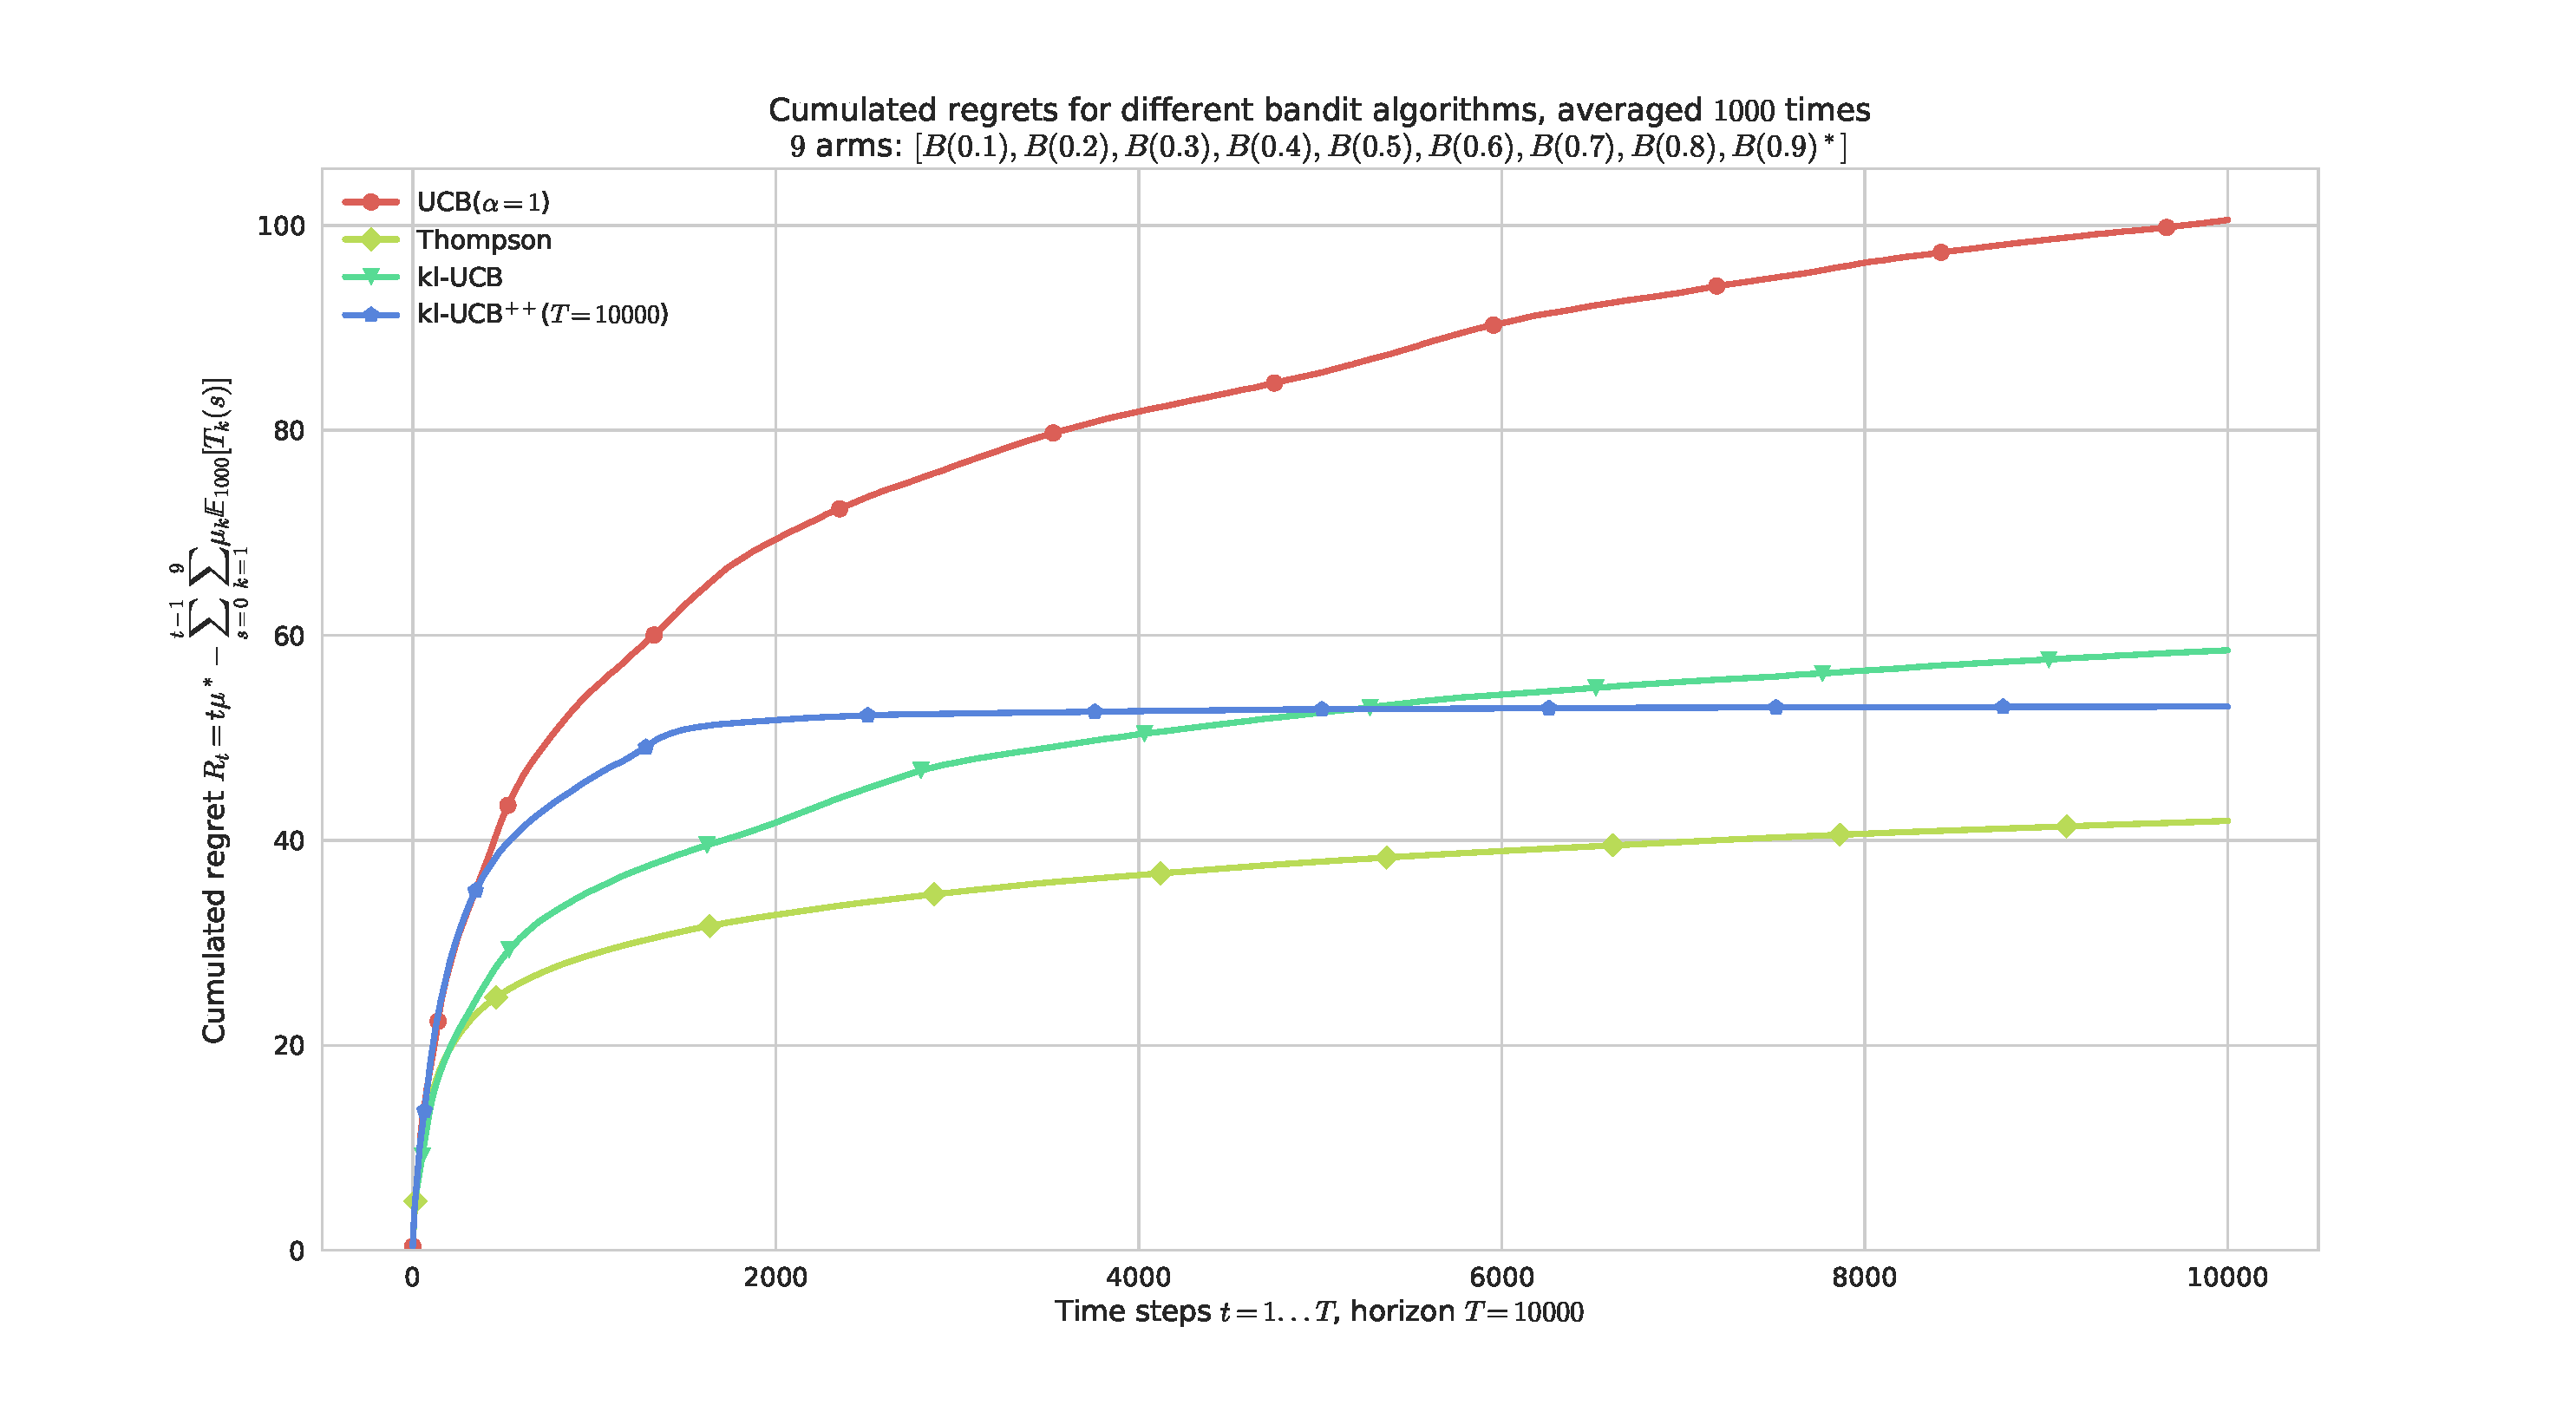
\includegraphics[width=1.15\textwidth]{../plots/paper/3.pdf}
\end{subfigure}
% ~ %add desired spacing between images, e. g. ~, \quad, \qquad, \hfill etc.
  %(or a blank line to force the subfigure onto a new line)
\begin{subfigure}[b]{0.49\textwidth}
  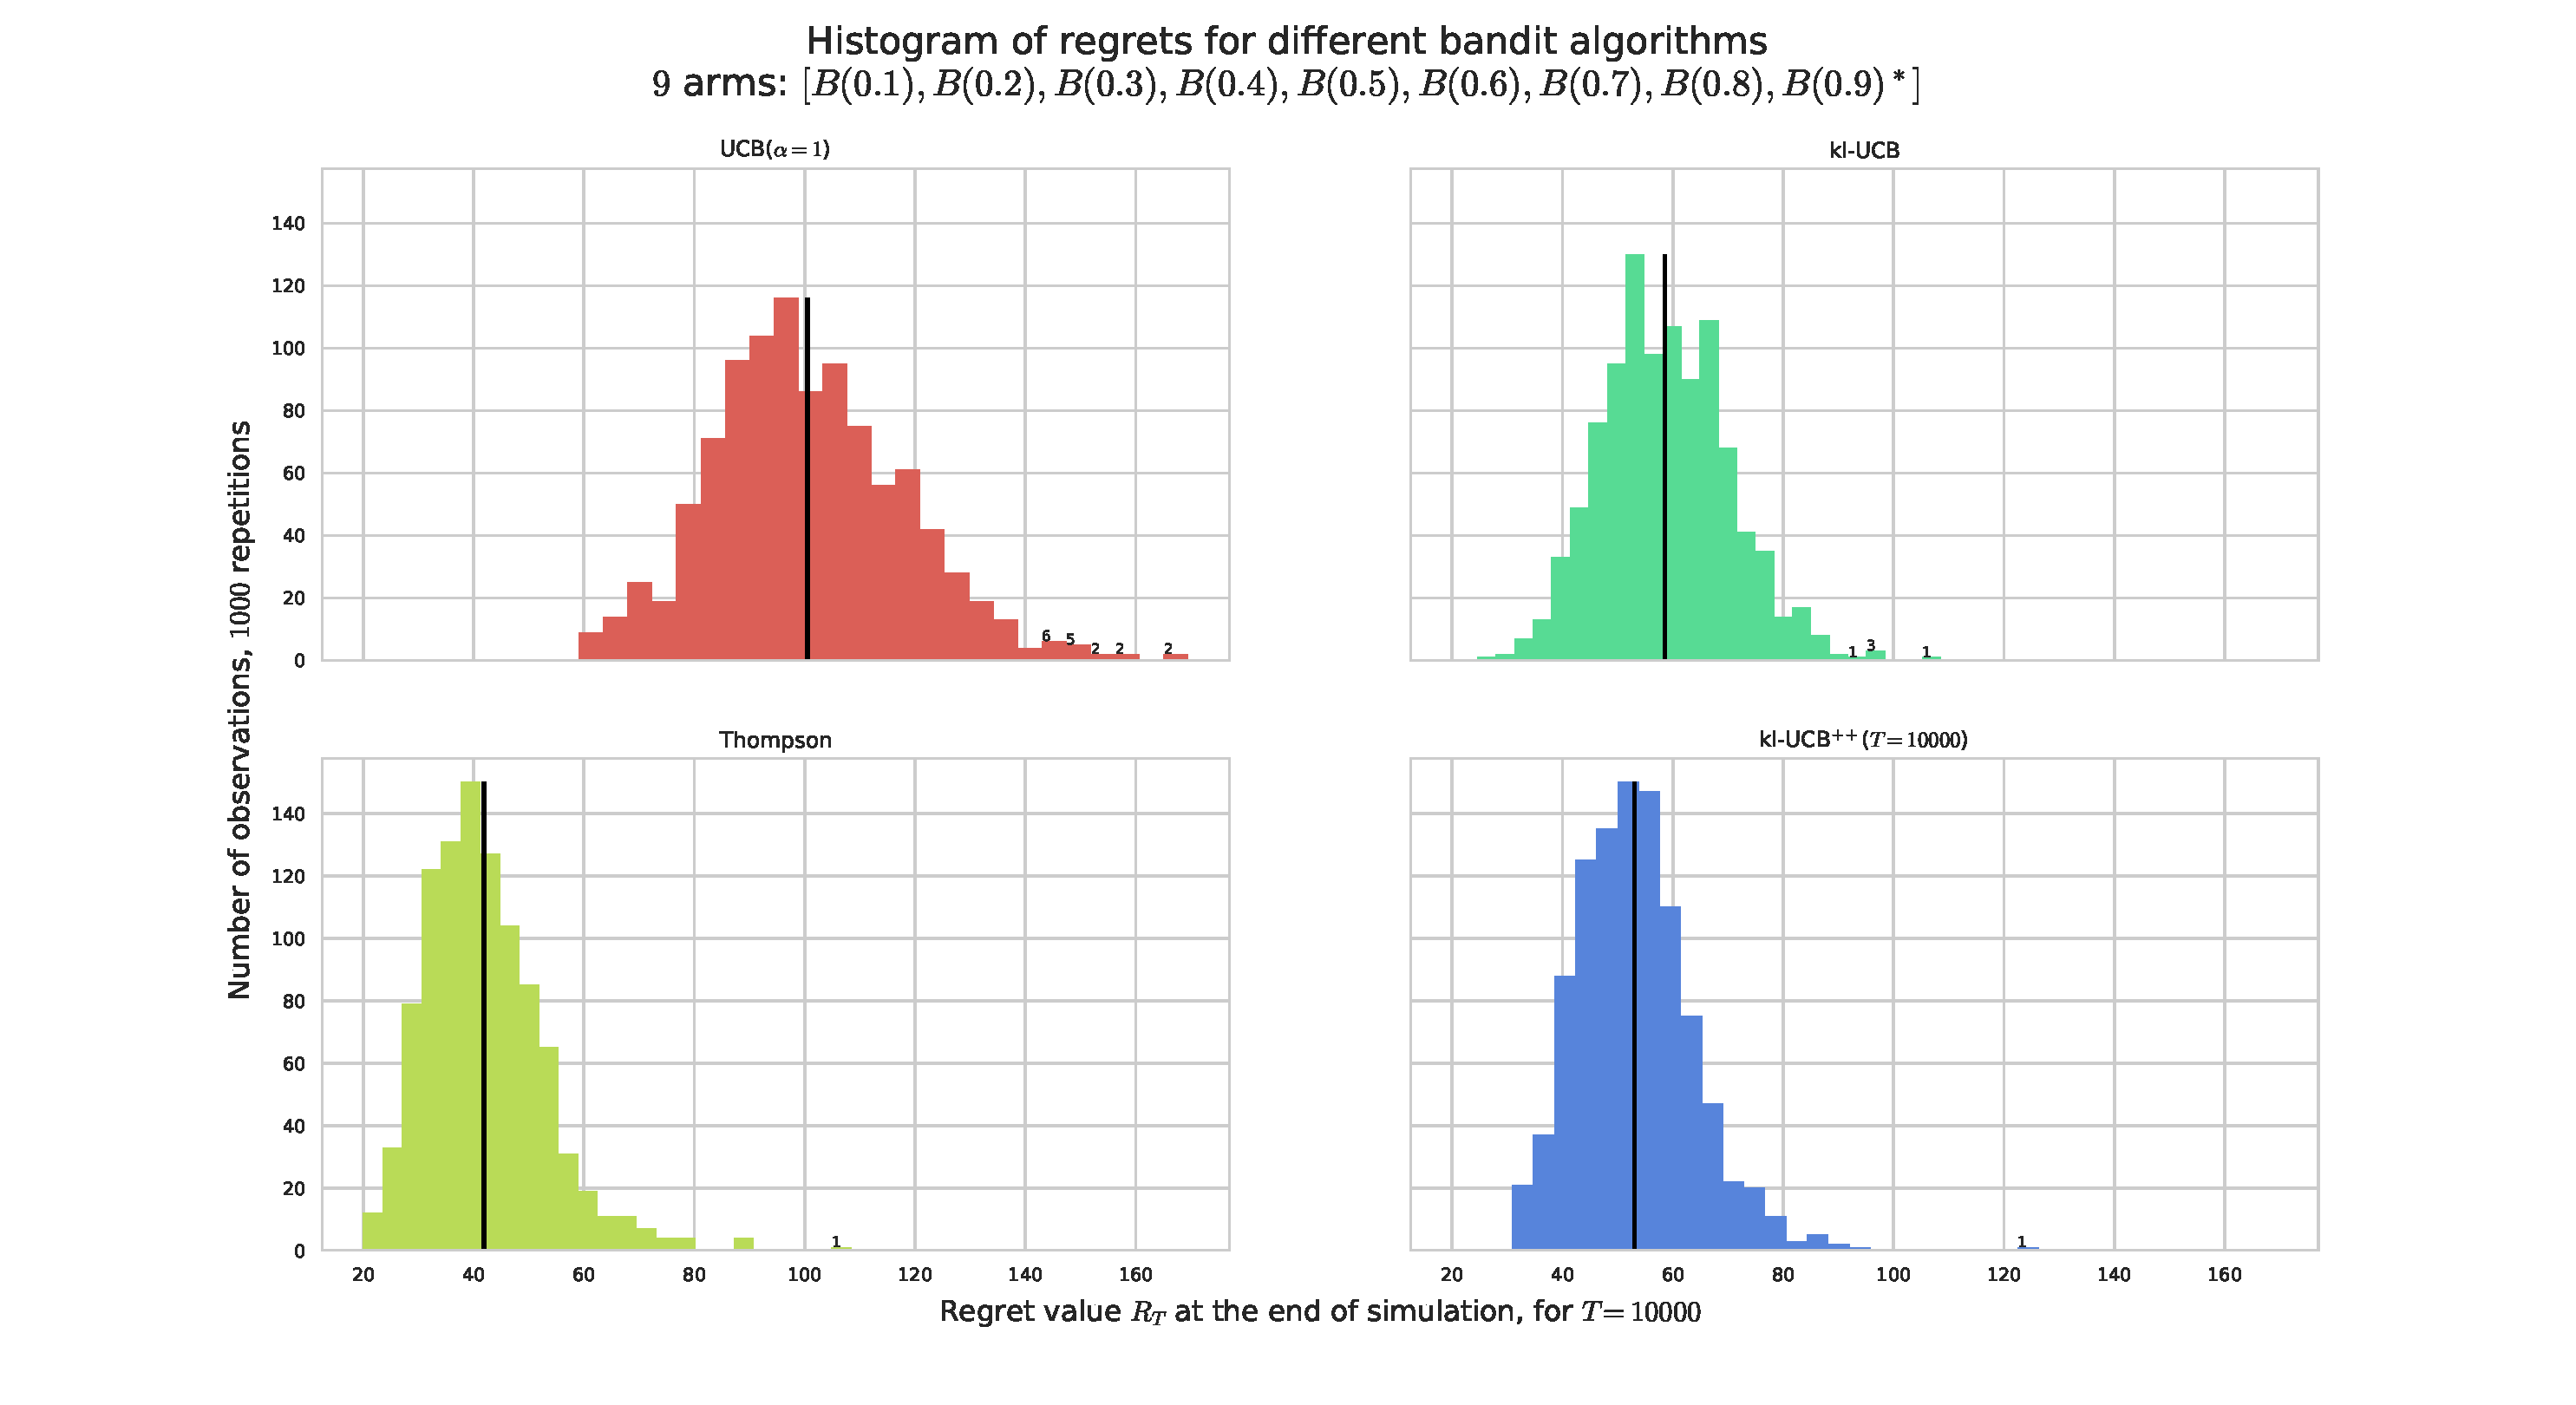
\includegraphics[width=1.15\textwidth]{../plots/paper/3_hist.pdf}
\end{subfigure}
\caption{Example of a single-player simulation showing the average regret and histogram of regrets of
\(4\) algorithms. They all perform very well: each algorithm is known to
be order-optimal (\emph{i.e.}, its regret is proved to match the
lower-bound up-to a constant), and each but UCB is known to be optimal
(\emph{i.e.} with the constant matching the
lower-bound). For instance, Thomson sampling is very efficient in average (in \textcolor{gold}{yellow}), and UCB shows a larger variance (in \textcolor{red}{red}).\label{fig:plot1}}
\end{figure}

% \begin{center}\rule{0.5\linewidth}{\linethickness}\end{center}

\section{\texorpdfstring{Research papers using \emph{SMPyBandits}}{Research using SMPyBandits}}\label{research-using-smpybandits}

\emph{SMPyBandits} was used for the following research articles since
\(2017\):

\begin{itemize}
\tightlist
\item
  For \citet{BessonALT2018}, we used \emph{SMPyBandits} for all the
  simulations for multi-player bandit algorithms\footnote{See
    the page
    \href{https://SMPyBandits.GitHub.io/MultiPlayers.html}{\texttt{SMPyBandits.GitHub.io/MultiPlayers}}
    on the documentation.}. We designed the two
  \href{https://SMPyBandits.GitHub.io/docs/PoliciesMultiPlayers.RandTopM.html}{\texttt{RandTopM}}
  and
  \href{https://SMPyBandits.GitHub.io/docs/PoliciesMultiPlayers.MCTopM.html}{\texttt{MCTopM}}
  algorithms and proved than they enjoy logarithmic regret in the usual
  setting, and outperform significantly the previous state-of-the-art
  solutions (\emph{i.e.},
  \href{https://SMPyBandits.GitHub.io/docs/PoliciesMultiPlayers.rhoRand.html}{\texttt{rhoRand}},
  \href{https://SMPyBandits.GitHub.io/docs/Policies.MEGA.html}{\texttt{MEGA}}
  and
  \href{https://SMPyBandits.GitHub.io/docs/Policies.MusicalChair.html}{\texttt{MusicalChair}}).
\end{itemize}

\begin{itemize}
\tightlist
\item
  In \citet{BessonWCNC2018}, we used \emph{SMPyBandits} to illustrate and
  compare different aggregation algorithms\footnote{See the page
    \href{https://SMPyBandits.GitHub.io/Aggregation.html}{\texttt{SMPyBandits.GitHub.io/Aggregation}}
    on the documentation.}. We designed a variant of the Exp3 algorithm
  for online aggregation (or boosting) of experts \citep{Bubeck12}, called
  \href{https://SMPyBandits.GitHub.io/docs/Policies.Aggregator.html}{\texttt{Aggregator}}.
  Aggregating experts is a well-studied idea in sequential learning and
  in machine learning in general. We showed that it can be used in
  practice to select on the run the best bandit algorithm for a certain
  problem from a fixed pool of experts. This idea and algorithm can have
  interesting impact for Opportunistic Spectrum Access applications
  \citep{Jouini09} that use multi-armed bandits algorithms for sequential
  learning and network efficiency optimization.
\end{itemize}

\begin{itemize}
\tightlist
\item
  In \citet{Besson2018DoublingTricks}, we used \emph{SMPyBandits} to illustrate and
  compare different ``doubling trick'' schemes\footnote{See the
    page
    \href{https://SMPyBandits.GitHub.io/DoublingTrick.html}{\texttt{SMPyBandits.GitHub.io/DoublingTrick}}
    on the documentation.}. In sequential learning, an algorithm is
  \emph{anytime} if it does not need to know the horizon \(T\) of the
  experiments. A well-known trick for transforming any non-anytime
  algorithm to an anytime variant is the ``Doubling Trick'': start with
  a horizon \(T_0\in\mathbb{N}^*\), and when \(t > T_i\), use
  \(T_{i+1} = 2 T_i\). We studied two generic sequences of growing
  horizons (geometric and exponential), and we proved two theorems that
  generalized previous results. A geometric sequence suffices to conserve minimax
  regret bounds (in \(R_T = \mathcal{O}(\sqrt{T})\)), with a constant
  multiplicative loss \(\ell \leq 4\), but cannot be used to conserve a
  logarithmic regret bound (in \(R_T = \mathcal{O}(\log(T))\)). And an
  exponential sequence can be used to conserve logarithmic bounds, with
  a constant multiplicative loss also \(\ell \leq 4\) in the usual
  setting. It is still an open question to know if a well-tuned
  exponential sequence can conserve minimax bounds, or even ``weak'' minimax
  bounds (in \(R_T = \mathcal{O}(\sqrt{T \log(T)})\)).
\end{itemize}

\section{Dependencies}\label{dependencies}

This library is written in Python \citep{python}, for versions \emph{2.7+} or \emph{3.4+},
using \texttt{matplotlib} \citep{matplotlib} for 2D plotting,
\texttt{numpy} \citep{numpy} for data storing, random number generations
and operations on arrays, \texttt{scipy} \citep{scipy} for
statistical and special functions, and \texttt{seaborn} \citep{seaborn}
for pretty plotting and colorblind-aware colormaps.

Optional dependencies include \texttt{joblib} \citep{joblib} for parallel
simulations, \texttt{numba} \citep{numba} for automatic speed-up on small
functions, \texttt{sphinx} \citep{sphinx} for generating the
documentation, and \texttt{jupyter}
\citep{jupyter} used with \texttt{ipython} \citep{ipython} to experiment
with the code.

% ---------------------------------------------
\begin{normalsize}
  \bibliography{paper.bib}
\end{normalsize}

\end{document}
